%!TEX root = ../main.tex



\section{Η υπέρυθρη ακτινοβολία}

\begin{figure}
  \centering
  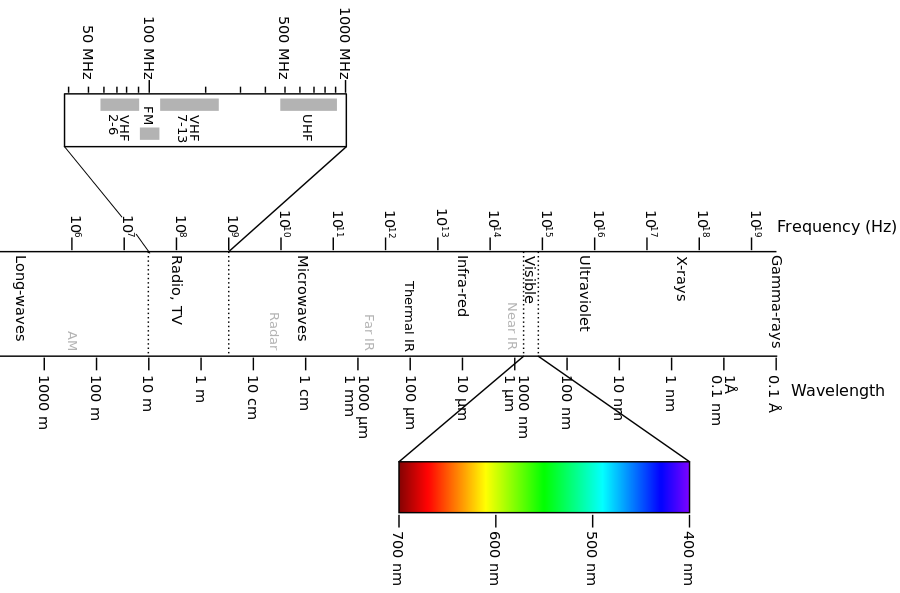
\includegraphics[width=\textwidth]{spectrum}
  \caption{Το φάσμα της Ηλεκτρομαγνητικής Ακτινοβολίας}
  \label{fig:spectrum}
\end{figure}


\lettrine[findent=2pt]{\fbox{\textbf{Ό}}}{πως} γνωρίζουμε από την επιστήμη της Φυσικής, όταν ένα σώμα ζεσταθεί αρκετά (π.χ. > 100 C) αρχίζει και εκπέμπει ακτινοβολία και στο οπτικό φάσμα (πέραν του υπέρυθρου), ενώ αποκτά ταυτόχρονα μια ερυθρή όψη. Κατά το φαινόμενο αυτό, η ακτινοβολια που εκπέμπεται ανήκει τόσο στο υπέρυθρο, όσο και στο ορατό φάσμα της ηλεκτρομαγνητικής ακτινοβολίας και μάλιστα το χρώμα που αποκτά το σώμα συνδέεται άμεσα με τη θερμοκρασία στην οποία βρίσκεται. Οι περιοχές της υπέρυθρης και ορατής ακτινοβολίας, καταλαμβάνουν τις ζώνες $1mm - 700nm$ και $700nm - 390nm$ αντίστοιχα, όπως φαίνεται και στο σχήμα \ref{fig:spectrum}.